%%%%%%%%%%%%%%%%%%%%%%%%%%%%%%%%%%%%%%%%%%%%%%%%%%%%%%%%%%%%%%%%%%%%%
% LaTeX Template: Project Titlepage Modified (v 0.1) by rcx
%
% Original Source: http://www.howtotex.com
% Date: February 2014
% 
% This is a title page template which be used for articles & reports.
% 
% This is the modified version of the original Latex template from
% aforementioned website.
% 
%%%%%%%%%%%%%%%%%%%%%%%%%%%%%%%%%%%%%%%%%%%%%%%%%%%%%%%%%%%%%%%%%%%%%%

\documentclass[12pt]{article}
\usepackage[a4paper]{geometry}
\usepackage[myheadings]{fullpage}
\usepackage{fancyhdr}
\usepackage{lastpage}
\usepackage{graphicx, wrapfig, subcaption, setspace, booktabs}
\usepackage[T1]{fontenc}
\usepackage[font=small, labelfont=bf]{caption}
\usepackage{fourier}
\usepackage[protrusion=true, expansion=true]{microtype}
\usepackage{sectsty}
\usepackage{commath}
\usepackage{url, lipsum}
\usepackage[utf8]{inputenc}
\usepackage{hyperref}
\usepackage[english]{babel}
\usepackage{csquotes}
\usepackage[sorting=none,backend=bibtex]{biblatex}
\addbibresource{cite.bib}

\newcommand{\source}[1]{\caption*{Source: \emph{#1}} }
\newcommand{\HRule}[1]{\rule{\linewidth}{#1}}
\onehalfspacing
\setcounter{tocdepth}{5}
\setcounter{secnumdepth}{5}

%-------------------------------------------------------------------------------
% HEADER & FOOTER
%-------------------------------------------------------------------------------
\pagestyle{fancy}
\fancyhf{}
\setlength\headheight{15pt}
\fancyhead[L]{Advanced problems in Computer Science}
\fancyhead[R]{Object Detection in Deep learning}
\fancyfoot[R]{\center{\thepage}}
%-------------------------------------------------------------------------------
% TITLE PAGE
%-------------------------------------------------------------------------------

\begin{document}

\title{ \normalsize \textsc{PROJECT REPORT\\
    Course: Advanced problems in Computer Science}
\\ [5.0cm]
\HRule{0.5pt} \\
\LARGE \textbf{\uppercase{OBJECT DETECTION IN DEEP LEARNING}}
\\ [0.25 cm]
\large {And their applications in real life}
\HRule{2pt} \\ [0.5 cm]
\normalsize  \vspace*{5\baselineskip}}

\date{
    \large{Academic year: 2020 - 2021}
}

\author{
    Dung Nguyen Manh \\
}

\newpage
\maketitle

%-------------------------------------------------------------------------------
% Section title formatting
\sectionfont{\scshape}
%-------------------------------------------------------------------------------

\newpage
\tableofcontents
\newpage

%-------------------------------------------------------------------------------
% ABSTRACTION
%-------------------------------------------------------------------------------

\begin{abstract}
For decades, people are dreaming about create a machine with the characteristics
of human intelligence, those can think and act like human. Nowadays, thanks to the
advancements of artificial intelligence and computational power, Computer Vision
technology has taken a big evolution and significant role in enabling digital
transformation across different industry. Computer Vision technology is
transformating the busniess world with its capability to understand the content
of digital images and videos. Accouding to Tractica \cite{tracitareport}, global
market for computer vision will increase from \$6.6 billion in 2015 to \$48.6
billion annually by 2022, which re-confirm the huge impact of Computer Vision fields
to this world. With the concept of capturing, processing, analyzing digital images
and videos, Computer Vision allows computer to see and understand the real world and
generates actionable insights as per designed algorithms. In this report, I will cover
the definition of Computer Vision and the most basic concept of its subfields,
especial Object Detection.
\end{abstract}

%-------------------------------------------------------------------------------
% INTRODUCTION
%-------------------------------------------------------------------------------

\section{INTRODUCTION TO COMPUTER VISION}
Computer Vision (CV) is a subfields of Aritficial Intelligence (AI), emerged in the
late 60’s and developed almost parallely with the AI field. 
The term "Computer Vision" have 2 components, where "Computer" refers an electronic 
machine capable of performing various processes, calculation, and operations from 
sets of instructions directed by software or hardware, and the term "Vision" refers
to visual perception throught sight where can be understand as the ability to "identify"
the objects located inside the environments. 

\begin{figure}[htp]
    \centering
    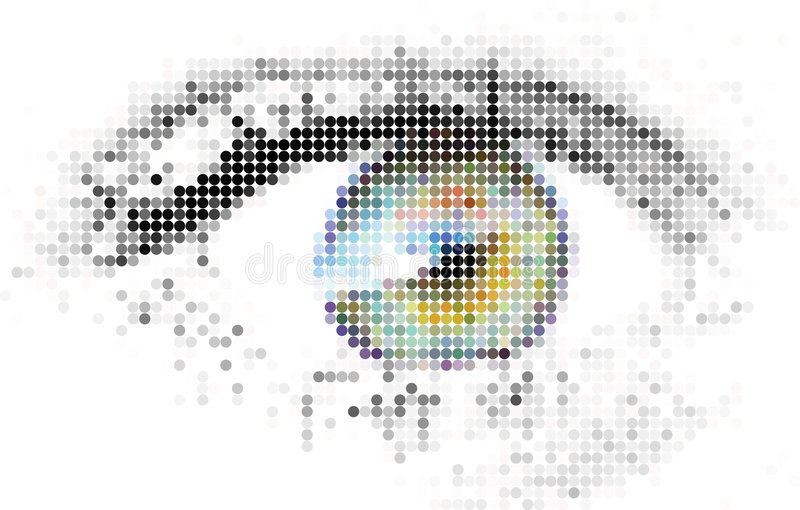
\includegraphics[width=0.5\textwidth]{images/digital-eyes.jpg}
    \caption{CV agent is an AI that can interpret and understand the visual world}
    \label{fig:computer_vision}
    \source{dreamstime.com}
\end{figure}

The concept of Computer Vision is based on teaching the machine how to “see” and 
interpret important information contained in images and videos. Computer Vision 
systems then use this translated data, 
using the knownledge provided by human beings, in order to improve the result of 
decision making process. Turning raw image data into higher-level concepts, that 
computers can interpret and act upon them is the principal goal of computer vision 
technology. 

\subsection{A brief history of Computer Vision}
Computer Vision is not new technology; the first experiments with Computer Vision 
started in the summer of 1966, Seymour Papert and Marvin Minsky started a project titled 
"Summer Vision Project" \cite{summervision}, where they built a system that can analyse 
a scence and identify objects in that scence. At that time, computer vision were relatively
simple and required a lot of work from human operators who had to provide data samples 
for analyse manually. It's hard to provide a decent amount of data, plus, the computational
power that day was not enough, therefore the error margin in this project was pretty high. 

\begin{figure}[htp]
    \centering
    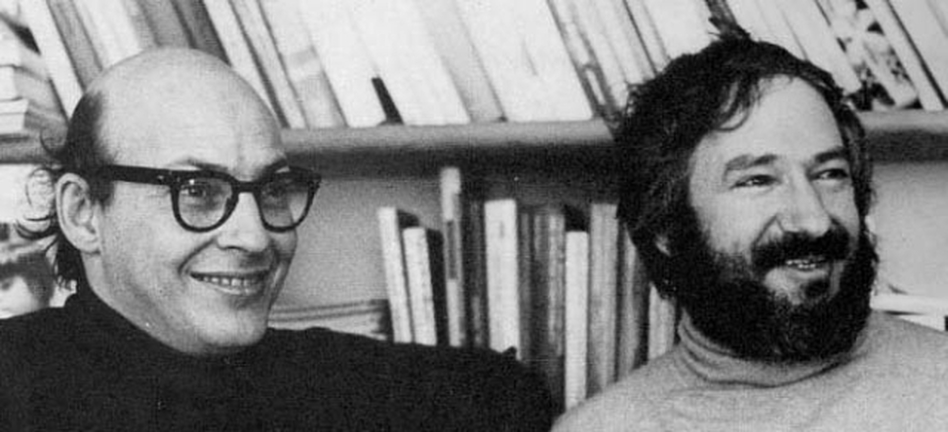
\includegraphics[width=0.9\textwidth]{images/minsky_papert.jpg}
    \caption{Seymour Papert and Marvin Minsky in The History of AI at AIWS.net}
    \label{fig:papert_minsky}
\end{figure}

At first, low-level tasks such as color segmentation or edge detection, etc, were already 
applied in the early day of the fields and formed the foundations of many mordern computer
vision this day. However, by the 80's, the scientific world generally agreed that the 
problem was not as trivial as they initially thought it was. Scientists quickly came to 
realise that tasks that are easily or even unconsciously done by humans are very difficult 
for a computer and the opposite. 

In late 70's and early 90's, knowns as "AI Winters", is a period of reduced funding and 
interest in artificial intelligence research \cite{aiwinter}. A principle, commonly known 
as Moravec’s paradox \cite{agrawal2010study}, was first formulated by the computer scientist 
Hans Moravec. Basically, it highlights that is much easier to implement specialized computers 
to mimic adult human experts (Deep Blue beat Kasparov at chess \cite{deepblue}) than building a 
machine with skills of 1-year old children with abilities to learn how to move around, 
recognize faces and voice or pay attention to interesting things. 

\begin{displayquote}[Moravec's paradox \cite{agrawal2010study}]
    Easy problems are hard and require enormous computation resources, 
    hard problems are easy and require very little computation. 
\end{displayquote}

The "winter" of connectionist research came to an end in the middle 1980s, 
when the work of John Hopfield, David Rumelhart and others revived large scale interest 
in neural networks. The mid 90's, the field has seen an increase in interest with the 
widespread use of machine learning and the first industrial applications. Scientists in Machine Learning started to 
shifts from a knowledge-driven approach to a data-driven approach, and many technical machine 
learning arrived such as Support-vector machines (SVM); Recurrent neural networks (RNN); etc.\cite{708428,medsker2001recurrent}
In the past decade, the introduction of deep learning has reinforced the interest in the field, 
intensifying the talk about an “AI spring”.

\subsection{Challenge in Computer Vision}
\label{sec:challenges}
The main purpose in development Computer Vision is not to imitate just human sight, but actually
to imitate the human visual perception. When parallelize the human visual system with 
the computer vision system, we can say both consist of sensor and interpreter. If our eyes
are our sensor that help us senses the light, then camera in many devices are machine 'eyes'.
The biggest challenge comes up with Computer Vision is not in machine eyes but the algorithm
teach them how to observate the world. 

\begin{figure}[htp]
    \centering
    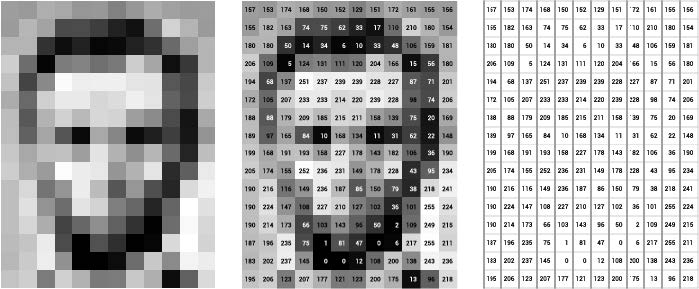
\includegraphics[width=0.9\textwidth]{images/how-computer-interpret-image.jpg}
    \caption{How computer interpret image}
    \label{fig:computer_image}
    \source{Openframeworks}
\end{figure}

A computer sees an image as series of pixels with it transforms to and array. 
The figure \ref{fig:computer_image} is a simple illustration of the grayscale image 
buffer which stores our image of Abraham Lincoln. 
Each pixel’s brightness is represented by a single 8-bit number, 
whose range is from 0 (black) to 255 (white). Nowadays, most of the images have 3
color channels which is RGB, then each channels no more represents grayscale intensity
but the related color intensity, eg: channels Red represents the intensity of color red 
in image. 

Because of the way computer or machine seeing the world, Computer Vision have to face 
many challenges. Therefore, it's not easy to answer what is the challenges in Computer 
Vision, these difficulties might vary from each to other fields in Computer Vision. 
The mose comman challenges in CV tasks such as objects under different viewpoints, 
illuminations, and intraclass variations, etc. 

Imagine we are building a Computer Vision system has ability to classify whether 
the objects in image are cat or not. That a look at a few example in figure \ref{fig:challenge} 
which can show us what type of difficulties that real life image 
bright to our model.
It's clearly that with the same cat, but if we change the camera angle, 
the system will definitely get another image which is unrelative to any other 
image that the system has seen.

\begin{figure}[htp]
    \centering
    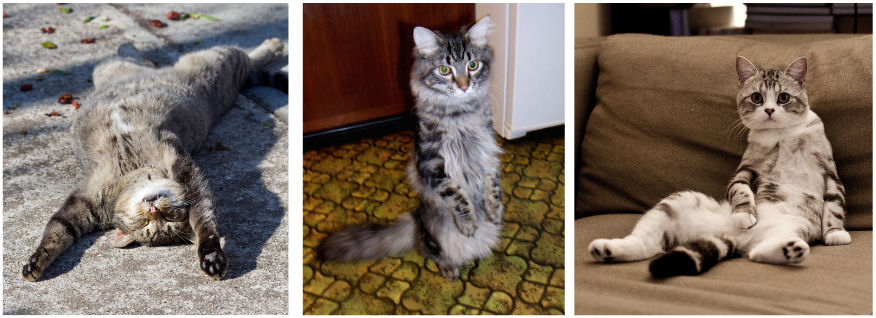
\includegraphics[width=0.9\textwidth]{images/cat_demo.png}
    \caption{Challenge on first day in Computer Vision }
    \label{fig:challenge}
    \source{CS231n Stanford}
\end{figure}

\section{WHAT IS OBJECT DETECTION}
We can not deny that Computer Vision, at the moments, take an important role in many 
applications. It takes part in many intelligence system that are able to understand and finish
their task through a process of interpreting the visual world by camera, videos, images, etc.
As one of the fundamental problems of computer vision, Object Detection form the basic 
of many other computer vision task, such as instance segmentation, image captioning, 
object tracking, etc. 

Object detection (OD) is a computer technology related image processing that deals 
with detecting instances of semantic objects of a certain class (such as humans, animals, or cars) 
in digital images and videos. 
The objective of object detection is to develop computational models and techniques that provide 
one of the most basic pieces of information needed by computer vision applications:
\emph{What objects are where?} 

While Object detection is a subfiled of computer vision, OD also face the most basic 
difficulties in computer vision that we covered in section \ref{sec:challenges}. However, 
object detection include (but not limited to) the following aspects: object rotation and
scale changes, accurate object localization, dense and occluded object detection, seed up of detection, etc. \\
Under the revolution of Deep learning, object detection has achieved many accomplishments.
Deep learning has lead object detection to remarkable breakthourgh and pushing it forward
to a research hot-spot with unprecedented attention. The number of publications
in object detection from 1998 to 2018 has increasing rapidly. \cite{zou2019object}

\begin{figure}[htp]
    \centering
    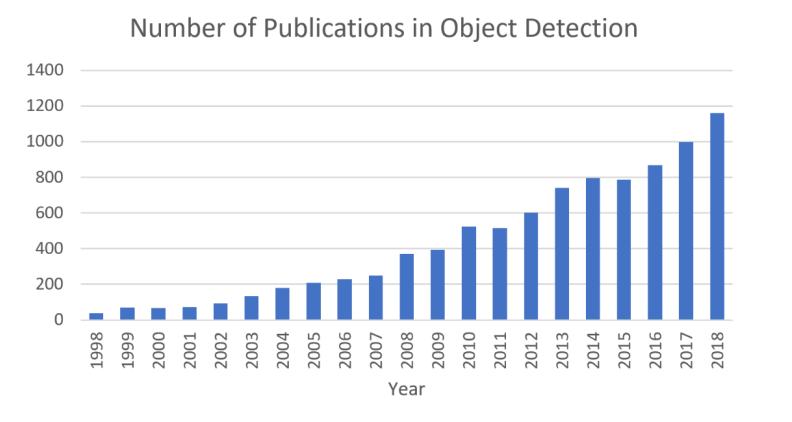
\includegraphics[width=0.75\textwidth]{images/number_of_publication.png}
    \caption{The increasing number of publications in object detection from 1998 to 2018}
    \label{fig:publication}
    \source{Object Detection in 20 Years: A survey \cite{zou2019object}}
\end{figure}

%-------------------------------------------------------------------------------
% A road map
%-------------------------------------------------------------------------------

\section{A ROAD MAP OF OBJECT DETECTION}
\label{sec:roadmap}
In the past two decades, the scientists widely argeed that object detection has 
gone through two historical periods: "traditional object detection" (before 2014)
and "deep learning based detection" (after 2014). 

\begin{figure}[htp]
    \centering
    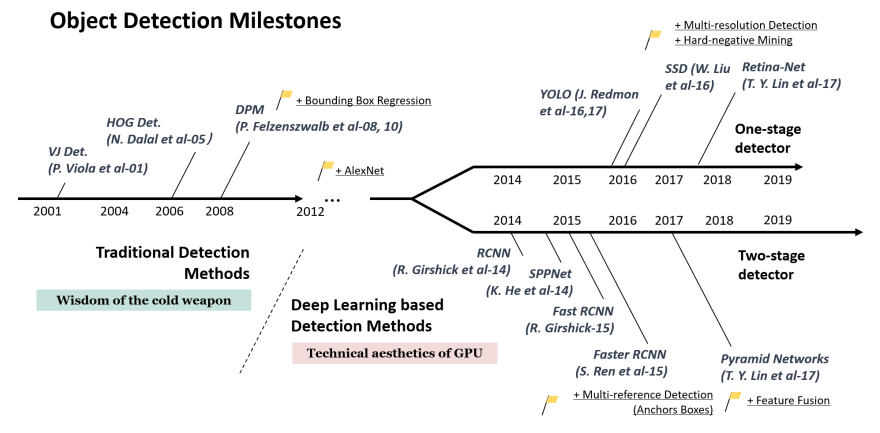
\includegraphics[width=1\textwidth]{images/roadmap.png}
    \caption{
        A road map of object detection. Milestone detectors in this figure: 
        VJ Det. \cite{viola2001rapid, viola2004robust}, 
        HOG Det. \cite{dalal2005histograms}, 
        DPM \cite{felzenszwalb2008discriminatively, felzenszwalb2010cascade, felzenszwalb2009object}, 
        RCNN \cite{girshick2014rich}, SPPNet \cite{he2015spatial},
        Fast RCNN \cite{wang2017fast}, 
        Faster RCNN \cite{ren2015faster}, 
        YOLO \cite{redmon2016you}, 
        SSD \cite{liu2016ssd}, 
        Pyramid Networks \cite{lin2017feature}, 
        Retina-Net \cite{lin2017focal}.
    }
    \label{fig:roadmap}
    \source{Object Detection in 20 Years: A survey \cite{zou2019object}}
\end{figure}

\subsection{Traditional Object Detectors}
\label{sec:tradional}
Turn back the clock 20 years, we would witness "the wisdom of cold weapon era". Most 
of the early object detection algorithms were built based on handcrafted features. 
Their performance easily stagnates by constructing complex ensembles which 
combine multiple low-level image features with high-level context 
from object detectors and scene classifiers. 

\subsubsection{Viola Jones Detectors}
\label{sec:viola}
Developed by Paul Viola and Michael Jones back in 2001 \cite{viola2001rapid}, 
the Viola-Jones Object Detection Framework can quickly and accurately 
detect objects in images and works particularly well with the human face.
The algorithm combines the concepts of Haar-like Features, Integral Images, 
the AdaBoost Algorithm, and the Cascade Classifier in order to create a system for 
object detection that is fast and accurate.

The VJ detector follows a most straight forward way of detection, i.e, sliding windows:
to go through all possible locations and scales in an image to see if any window might 
contains a human face. Althought it seems to be a very simple process, the calculation 
behind it was far beyond the computer's power of its time.
The VJ detector has dramatically improved its detection speed by incorporating three 
important techniques: "integral image", "feature selection", and "detection cascades".
While the VJ detector was tens or even hundreds of times faster than any other algorithms in its 
time under comparable detection accuracy, but in the scope of 
this report, I will not get deeper in detail of how VJ detector work.
\begin{figure}[htp]
    \centering
    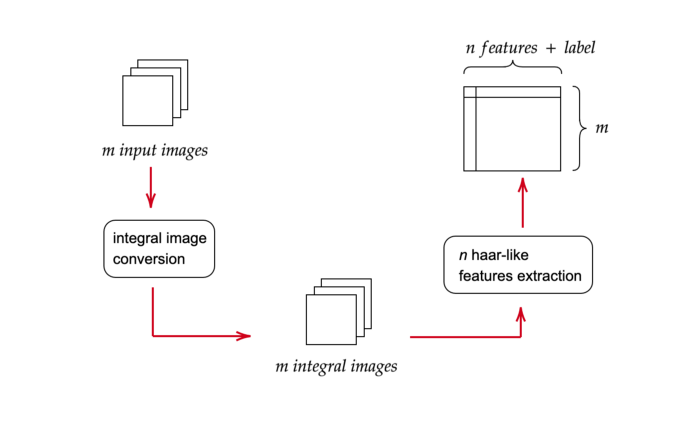
\includegraphics[width=0.8\textwidth]{images/vj_detector_process.png}
    \caption{Integral image and how Haar exacting features}
    \label{fig:haar}
    \source{Socret Lee (towardsdatascience.com)}
\end{figure}

\subsubsection{Histogram of Oriented Gradients (HOG) Detector}
\label{sec:hog}
Release by N. Dalal and B. Triggs in 2005 \cite{dalal2005histograms}, the HOG methods,
Histogram of Oriented Gradients, were considered as an important improvement of the 
scale-invariant feature transform and shape contexts of its time. The core of HOG 
algorithm is image gradient vector. It's a metric for every individual pixel, containing
the pixel color changes in both x-axis and y-axis which represent the dirrection of colors 
changing from one extreme to the other. 
\begin{figure}[htp]
    \centering
    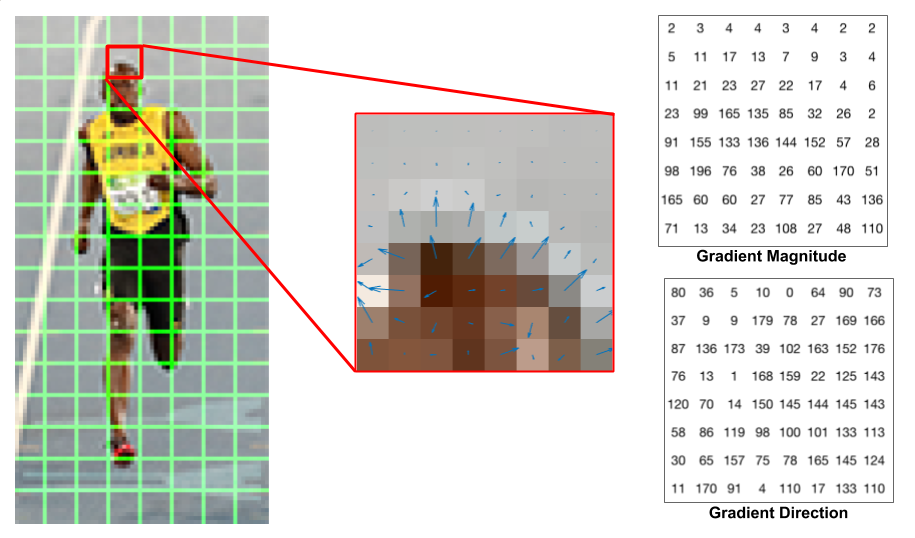
\includegraphics[width=0.8\textwidth]{images/vector_gradient.png}
    \caption{Visuallization of image gradient vector}
    \label{fig:gradient}
    \source{learnopencv.com}
\end{figure}

The HOG descriptor is designed to compute the gradient vector of every pixel 
on a dense grid of uniformly spaced cells. Then it searchs for all possible regions 
that counld contains object in images and use overlapping local contrast normalization 
(on block) for improving accuracy. To able to detect objects of different size, the 
HOG detector rescales the input image for multiple times while keeping the size of 
detecting window unchanged.

\subsubsection{Deformable Part-based Model (DPM)}
\label{sec:dpm}
DPM was originally proposed by P.Felzenswalb in 2008 \cite{felzenszwalb2008discriminatively}
as an extension of the HOG detector. The PASCAL Visual Object Classes Challenge 2007, 
2008 and 2009 pronounce DPM as the winners, therefore, it can be called as the peak 
of the traditional object detection methods. 

Followings the detection philosophy of "divide and conquer", where the training can 
be simply considered as the learning of a proper way of decomposing an object. 
and the inference can be considered as an ensemble of detections on different object 
parts. For example, when detecting a "bicycle" can be considered of detecting wheels, 
body. This was named "star-model" published by P. Felzenszwalb \cite{felzenszwalb2008discriminatively}.

\begin{figure}[htp]
    \centering
    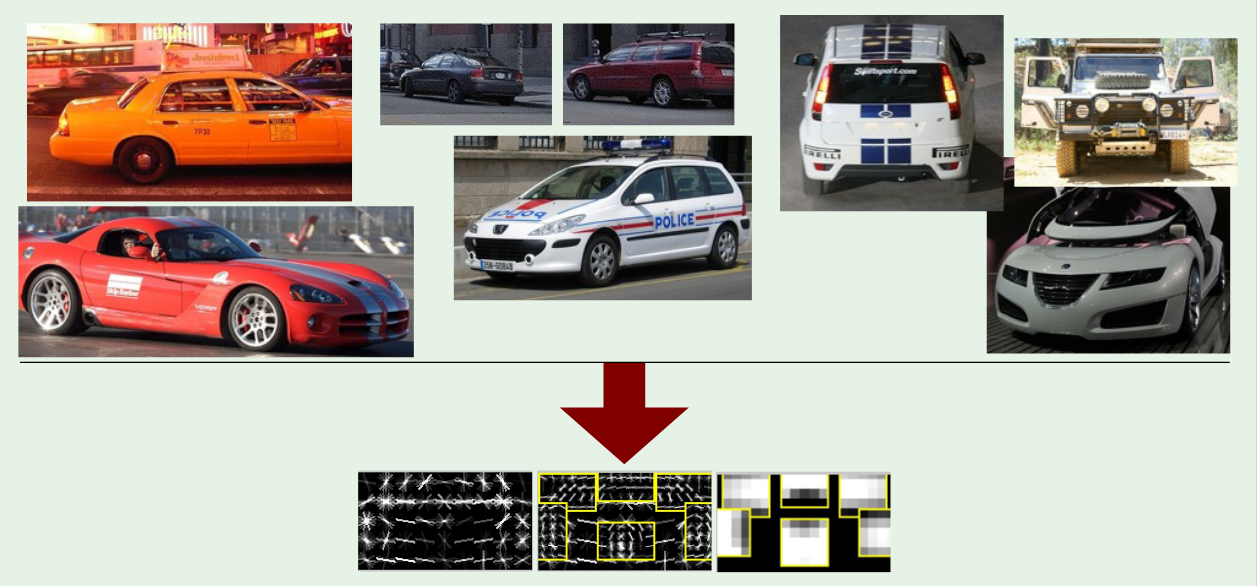
\includegraphics[width=1\textwidth]{images/dpm.png}
    \caption{Root-filter and part-filters of a car in DPM algorithm}
    \label{fig:dpm}
    \source{CS231b Stanford}
\end{figure}

A typical DPM detector consists of a root-filter and a number of part-filters. Instead 
of manually specifying the configurations of the part filters. Instead of manually 
specifying the configurations of the part filters (e.g., size, location), a weakly supervised 
learning method is developed in DPM where all configurations of part filters can be 
learned automatically.



\subsection{Deep Learning based Detection}
\label{sec:deep_learning}

\subsubsection{CNN based Two-stage Detectors}
\label{sec:two_stage}

\subsubsection*{RCNN}
\subsubsection*{Fast RCNN}
\subsubsection*{Faster RCNN}

\subsubsection{CNN based One-stage Detectors}
\label{sec:one_stage}

\subsubsection*{You Only Look Once (YOLO)}
\subsubsection*{Single Shot MultiBox Detector (SSD)}

%-------------------------------------------------------------------------------
% DISCUSSION
%-------------------------------------------------------------------------------

\section{OBJECT DETECTION IN FUTURE}
\label{sec:future}
\subsection{Ethical issues in Object Detection}
\label{sec:ethical}
% add current ethical issues in OD
% personal privacy, information security, crimial tracking or citizen tracking?
% deep fake, bla bla
\subsection{Object Detection current and future trends}
\label{sec:trend}


%-------------------------------------------------------------------------------
% REFERENCES
%-------------------------------------------------------------------------------
\newpage
\printbibliography

\end{document}
